%%%%%%%%%%%%%%%%%%%%%%%%%%%%%%%%%%%%%%%%%%%%%%%%%%%%%%%%%%%%%%%%%%%%%%%%%%%%%%%%
%2345678901234567890123456789012345678901234567890123456789012345678901234567890
%        1         2         3         4         5         6         7         8

\documentclass[letterpaper, 10 pt, conference]{ieeeconf}  % Comment this line out
                                                          % if you need a4paper
%\documentclass[a4paper, 10pt, conference]{ieeeconf}      % Use this line for a4
                                                          % paper

\IEEEoverridecommandlockouts                              % This command is only
                                                          % needed if you want to
                                                          % use the \thanks command
\overrideIEEEmargins
% See the \addtolength command later in the file to balance the column lengths
% on the last page of the document

%\addtolength{\textheight}{-3cm}   % This command serves to balance the column lengths
                                  % on the last page of the document manually. It shortens
                                  % the textheight of the last page by a suitable amount.
                                  % This command does not take effect until the next page
                                  % so it should come on the page before the last. Make
                                  % sure that you do not shorten the textheight too much.



% The following packages can be found on http:\\www.ctan.org
\usepackage{graphicx} % for pdf, bitmapped graphics files
%\usepackage{epsfig} % for postscript graphics files
%\usepackage{mathptmx} % assumes new font selection scheme installed
\usepackage{times} % assumes new font selection scheme installed
\usepackage{amsmath} % assumes amsmath package installed
\usepackage{amssymb}  % assumes amsmath package installed
\usepackage{float}
\usepackage{url}
\usepackage{tikz}
\usepackage{subfigure}
\usepackage{textcomp} % a whole package to get the \textdegree symbol. 
%\usepackage{savetrees}

\usepackage{subfigure} 

\title{\LARGE \bf Learning a Wall Following Behavior using\\ Sarsa($\lambda$) Reinforcement Learning}

%\author{ {\centering John R. Hoare
%         \thanks{J. R. Hoare is with the Distributed Intelligence Laboratory, Department of Electrical Engineering and %Computer Science, University of Tennessee, Knoxville, TN 37996-3450, jhoare@eecs.utk.edu.}}
%}

\author{John Hoare\\% <-this % stops a space
Distributed Intelligence Laboratory, Department of Electrical Engineering and Computer Science\\
The University of Tennessee, Knoxville, TN 37996-3450\\
Email: jhoare@eecs.utk.edu
}

% Allow big floats to be put at the bottom of the page
%\renewcommand{\topfraction}{0.95}
%\renewcommand{\bottomfraction}{0.95}
%\renewcommand{\floatpagefraction}{1.00}
%\renewcommand{\textfraction}{0.1}
%\addtolength{\dbltextfloatsep}{-1in}
%\addtolength{\floatsep}{-0.2in}

\renewcommand\floatpagefraction{.9}
\renewcommand\topfraction{.9}
\renewcommand\bottomfraction{.9}
\renewcommand\textfraction{.1}   
\setcounter{totalnumber}{50}
\setcounter{topnumber}{50}
\setcounter{bottomnumber}{50}

\begin{document}



\maketitle
\thispagestyle{empty}
\pagestyle{empty}


%%%%%%%%%%%%%%%%%%%%%%%%%%%%%%%%%%%%%%%%%%%%%%%%%%%%%%%%%%%%%%%%%%%%%%%%%%%%%%%%
\begin{abstract}
In this work a simulated robot learns to follow a wall by using the reinforcement learning technique Sarsa($\lambda$). 
The robot uses a 180 degree laser scanner mounted at 45 degrees to the left, which the robot uses to follow the left-hand side wall. 
The robot successfully learns a control that enables it to follow the wall on the left side.
Presented is the discritation method for the state-space, as well as the situations presented to the robot in order to have it learn.
\end{abstract}


%%%%%%%%%%%%%%%%%%%%%%%%%%%%%%%%%%%%%%%%%%%%%%%%%%%%%%%%%%%%%%%%%%%%%%%%%%%%%%%%
\section{Introduction}
In this paper work is presented that enables a robot simulated in the stage environment to follow walls along its left side. 
The robot learns this behavior using the Sarsa($\lambda$) reinforcement learning algorithm. 
\subsection{Problem Formulation}
For this work, the robot is assumed to begin along-side a wall, and must continue to follow the wall. 
The robot will not start in free-space and "search" for the wall. 
The desired distance from a wall is denoted with $\delta_w$ which is set to 0.75 meters. 
Additionally, the robot is considered to be within this distance if it is within $\epsilon_w = 0.25$ meters of $\delta_w$.

%%%%%%%%%%%%%%%%%%%%%%%%%%%%%%%%%%%%%%%%%%%%%%%%%%%%%%%%%%%%%%%%%%%%%%%%%%%%%%%%
\section{Approach}
Reinforcement learning relies on learning the optimum action given a specific state. 
In this section a definition of how the current state is determined, and what the available actions are.
\subsection{Robot}
The robot is a pioneer 3dx robot, with a mounted sick lms200 laser range finder, mounted 45\textdegree to the left.
The robot has other sensors also available to it, however only the laser range finder is used for this work.
\subsection{States}
The laser range finder provides far too much information directly to have a discrete state space. 
Because of this the laser is used to create a much smaller, discrete state space. 
While, the laser returns a range to an obstacle, this needs to be much more simple for a discrete state space.
Because of this, we convert the range readings to discrete measurements: 
\begin{align}
\text{d-range}(r) &= \left\{ \begin{array}{ll} 
\text{LOW} & \mbox{if $r < \delta_w - \epsilon_w$} \\
\text{GOOD} & \mbox{if $ (\delta_w -\epsilon_w) \geq r \geq (\delta_w + \epsilon_w)$} \\
\text{HIGH} & \mbox{if $r > \delta_w + \epsilon_w$} \\
\end{array} \right.
\end{align}
The laser is cut into four regions total, first dividing the laser into thirds, and then sub-dividing the frontward-facing third again into half, where the minimal range value from each region is used as the representative laser range. 
From this, we create a four-tuple that represents the current state.
\begin{align}  
S_{\text{region}} &= \min_{i \in \text{region}} \text{d-range}(r_i) \, \, \forall \text{ region}
\end{align}
Because there are four regions, and three possible ranges (values) for each region, there is a total of $3^{4} = 81$ states.
The duration of a state is 5 player robot.Read() cycles, which occur at 20Hz.
This results in a state lasting approximately $\frac{1}{4}$ of a second. 

\begin{figure}
\centering
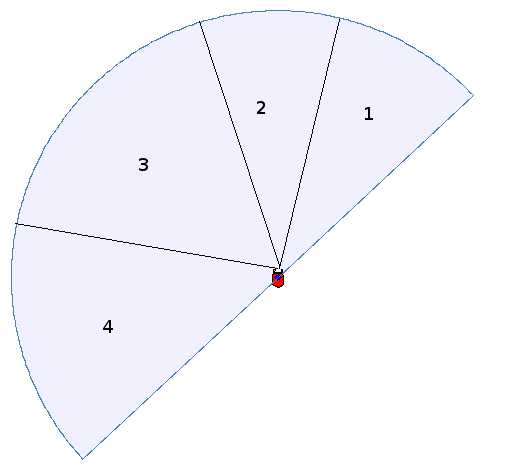
\includegraphics[width=2.5in]{statespace.png}
\caption{The configuration of the robot and a graphical representation of how the laser is split up. 
Region 4 is the so-called ``goal'' region, that is the region that the robot tries to keep a distance of $\delta_w$ away.}
\label{fig:statespace}
\end{figure}

\begin{figure}
\centering
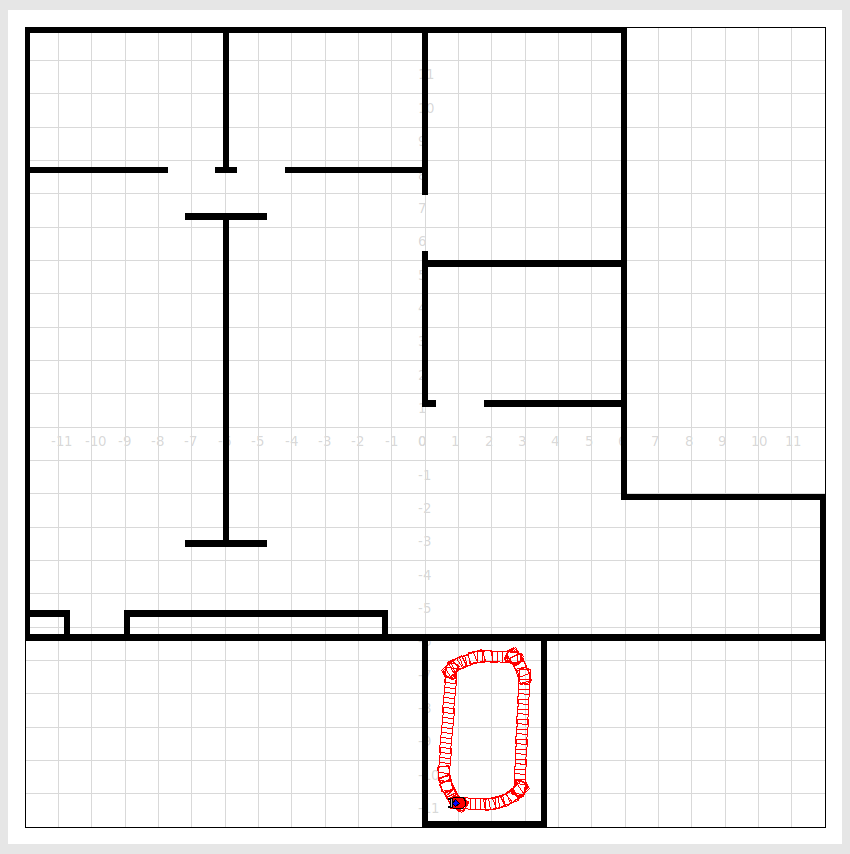
\includegraphics[width=2.5in]{stage-in-smallroom.png}
\caption{The robot first learns to follow the wall in a small, simple environment.
Results shown are after 600 epsiodes.}
\label{fig:smallroom}
\end{figure}


\subsection{Actions}
To keep the learning task more tractable, a minimal set of actions are defined. 
The robot has a turn left/right action as well as a drive forward action. 
The turn left and turn right actions both have a very minor forward component, to be able to move the robot out of oscillatory behavior. 
With 81 states, and 3 actions, the size of $Q$ becomes $81\times3$. 
\subsection{Reward Function}
The reward function is defined as a function of both the state and action. 
The state has a ``reward'' region, which is the region that the robot is to try to keep within the GOOD distance. 
The reward function gives the maximum reward, if the robot is within that state, and is executing the ``move forward'' action. 
The reward function is explicitly defined as: 
\begin{align}
\text{reward}(s,a) &= \left\{ \begin{array}{ll}
-10 & \mbox{if stalled} \\
-1 & \mbox{if $\exists$ LOW $\in s$} \\
 2 & \vbox{\hbox{if $s_{\text{reward}} = \text{GOOD}$}
 			\vspace{2pt}
              \hbox{\& $a = $ FORWARD}}  \\
 0.25 & \mbox{if $s_{\text{reward}} = \text{GOOD}$} \\
 -1 & \mbox{if left the reward region}
\end{array}
\right.
\end{align}

\subsection{Constants}
Provided in Table~\ref{Table:constants} are the constants used in the learning activity. 
$\epsilon$ is different depending on which stage of training currently in (see next section) and decays by multiplying the last epsilon by 0.999 at the end of each episode. 

\begin{table}
\centering
\caption{Constant values used in Sarsa($\lambda$)}
\label{Table:constants}
\begin{tabular}{|c|c|}
\hline
Constant & Value \\
\hline \hline
$\lambda$ & 0.9 \\
\hline 
$\gamma$ & 0.1 \\
\hline
$\alpha$ & 0.1 \\
\hline
\end{tabular}
\end{table}



\subsection{Training Method}
Training is done by starting the robot next to the wall about $\delta_w$ distance away, and an episode lasts as long as the robot travels without hitting a wall, or wandering away from the wall. 
At first, training is done in an epsilon-greedy fashion, where the robot is in a small, enclosed room shown in figure~\ref{fig:smallroom}. 
The robot trains within the small room for approximately 4 hours, or 600 episodes. 
Once the robot is able to wall-follow in the small room the next stage of training begins.
The robot is put into the normal environment, and trains for several more hours, using a strictly greedy approach. 
During this time, an epoch will last for much longer, as the robot is much more close to an optimum policy, and will make mistakes much more rarely. 
As time pasts, the robot learns to travel through the entire environment, avoiding obstacles. 
The robot experiences 48 more episodes over about 18 hours of training, to learn an effective policy. 
Of course the exact times and number of episodes will vary due to randomness, but the reported times are given as a guide. 

%%%%%%%%%%%%%%%%%%%%%%%%%%%%%%%%%%%%%%%%%%%%%%%%%%%%%%%%%%%%%%%%%%%%%%%%%%%%%%%%
\section{Evaluation}
As the robot was trained as explained in the previous section, the state was stored at every 50 training episodes. 
From the states, we can plot the learned reward function, which can visualize how the robot is able to learn the optimum policy over time. 
The learned policy is also tested in a less structured, ``hospital'' environment, to see how well of a policy is learned for more complicated worlds. 



\begin{figure*}
\centering
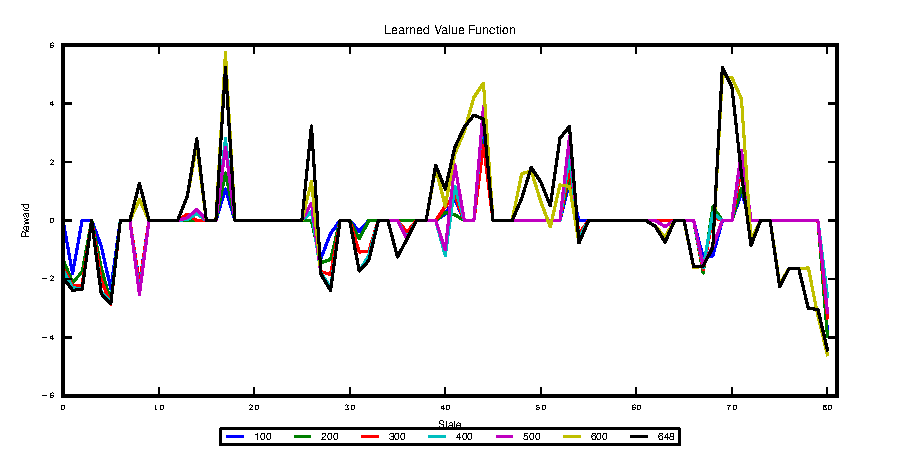
\includegraphics[width=6in]{value-func.pdf}
\caption{The learned value function, after different levels of episodes.}
\label{fig:value-func}
\end{figure*}

\begin{figure}
\centering
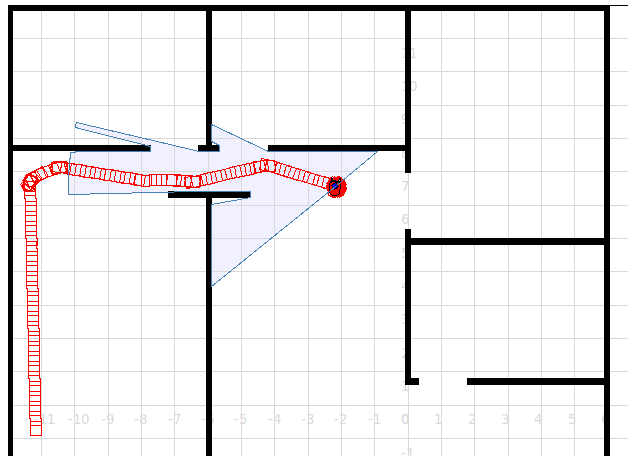
\includegraphics[width=2.5in]{stage-after-smallroom.png}
\caption{The robot moving in the full environment, after it has only been experimenting within the smaller environment.
The robot is unable to sucessfully follow the wall through the full envionment, and fails to enter the two top rooms. 
Results shown are after 600 epsiodes.}
\label{fig:smallroom}
\end{figure}

\begin{figure}
\centering
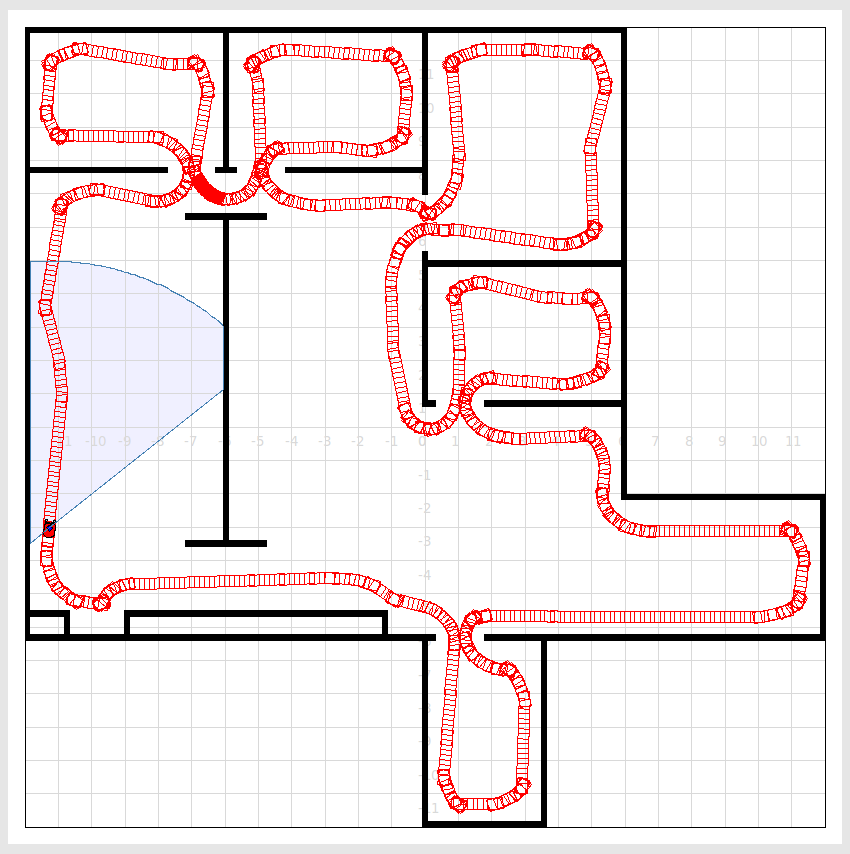
\includegraphics[width=2.5in]{stage-full-learned.png}
\caption{The robot moving in the full environment, after it has learned its final policy. 
The robot is able to successfully navigate through the environment, entering any rooms it goes by. 
In the narrow hallway above, the robot participates oscillatory behavior, which causes it to move very slowly through this area.}
\label{fig:full-learned}
\end{figure}

\begin{figure}
\centering
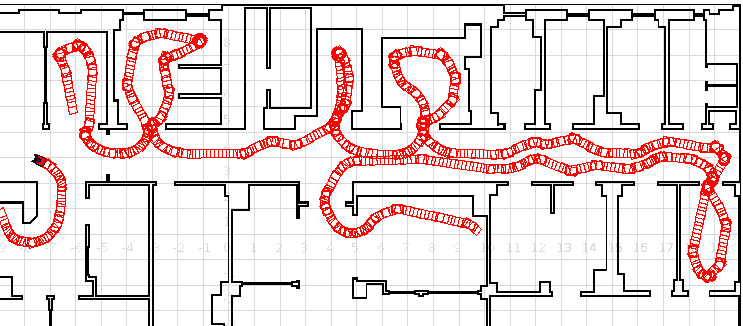
\includegraphics[width=2.5in]{hospital.png}
\caption{The robot moving in the more complex, ``hospital'' enviornment, after it has learned its final policy from the other environment. 
The robot is able to usually wall-follow successfully, however it us unable to enter the small doors, and will sometimes collide with the walls in some of the more complicated rooms. }
\label{fig:hospital}
\end{figure}


%%%%%%%%%%%%%%%%%%%%%%%%%%%%%%%%%%%%%%%%%%%%%%%%%%%%%%%%%%%%%%%%%%%%%%%%%%%%%%%%
\section{Results}
After 648 training episodes (about 22 hours), the robot is able to follow the wall without collisions as shown in Figure~\ref{fig:full-learned}. 
While the robot goes through the hallway at the top of the map, it exhibits oscillatory behavior, but is however able to overcome this due to the slight forward action that is in the turn left/right methods. 
The learned value function is shown in figure~\ref{fig:value-func}. 
In the value function any state that is 0 is either no reward, or more likely an unvisited state. 
It is likely that there are many ``useless'' states that are not necessary when the robot starts next to the wall, that the robot does not encounter in the more simple environment, and as we can see from Figure~\ref{fig:full-learned}, the robot is still very much able to preform well without knowledge of these states.


%%%%%%%%%%%%%%%%%%%%%%%%%%%%%%%%%%%%%%%%%%%%%%%%%%%%%%%%%%%%%%%%%%%%%%%%%%%%%%%%
\section{Conclusions and Future Work}
The robot has successfully learned to follow the wall by using the Sarsa($\lambda$) reinforcement learning technique.
This work has presented a method to iteratively train the robot to handle more and more complicated environments, in order to allow the robot to more slowly encounter new things.
This method gives the robot a more likely chance to be able to succeed or to learn how to handle the new abnormality in the environment.  
The forward most region was divided into two (from the original 3 regions to 4 regions) to try to deal with the oscillatory behavior exhibited in the hallway. 
The oscillatory behavior is lessened by the increased state space but is still there, it is likely that further subdivisions may help, however it will also likely cause the learning time to go higher.
Also, changing the reward function so the robot gets no reward while turning may also help stop this oscillatory behavior.
In the hospital environment, the robot encounters many of the aforementioned "0" states, and the robot is unable to pick a good action. 
Future work would be to develop a way for the robot to encounter these states and be able to do exploration only at these points. 
Classical $\epsilon$-greedy methods would not allow the robot to get far enough. 
A likely good solution, would be to have a step where the robot wanders around using its learned policy, and save the position of the robot a few seconds before failing (impacting a wall), and use this to generate initial positions for the robot to then follow an $\epsilon$-greedy approach to learn how to handle these new instances. 


%%%%%%%%%%%%%%%%%%%%%%%%%%%%%%%%%%%%%%%%%%%%%%%%%%%%%%%%%%%%%%%%%%%%%%%%%%%%%%%%


\bibliographystyle{plain}
%\bibliography{neural_net}

\end{document}

